\documentclass[a4paper, 12pt]{report}

\usepackage{color}
\usepackage{graphicx}
\usepackage{subcaption}
\usepackage{amsmath} 

\begin{document}

\title{Speech Emotion Recognition Using Deep Learning}
\author{Jakir Hasan - 2018331057}
\date{30 December 2022}
\maketitle
\pagenumbering{roman}
\newpage
\pagenumbering{arabic}
\setcounter{chapter}{1}

\section{Abstract}
In this study, we have presented a deep learning-based implementation for speech emotion recognition (SER). The system uses a Multilevel Perceptron Classifier. The proposed model has been applied to SUBESCO dataset. The experimental results reveal that the model with MLPClassifier achieves better performance. The proposed model has attained a weighted accuracy (WAs) of 77\% for the SUBESCO dataset.

\section{Index Term}
SER, MLPClassifier, SUBESCO

\section{Introduction}
Though a lot of work has been done in the area of Speech Emotion Recognition (SER) , there is still a lot of scope to improve. Researchers have developed many tools and techniques to classify emotions from speech signals. These tools and techniques are mainly developed for languages such as English, German, French etc. But there is not much progress for low resource languages such as Bangla.\\\\
Keeping these in mind we have implemented a deep learning based Multi Level Perceptron Classifier (MLPClassifier) to classify human emotions from Bengali audio speech signals. We used the SUBESCO dataset developed by SUST. \\\\
We also developed a web application where users can provide audio files or record audio and can show predicted emotion.\\


\section{Problem Definition}
Speech signals contain a lot of valuable information in it. Extracting the right features from speech signals is tricky and difficult. For predicting emotions we have to extract features which give high quality information. So, the main problem is to extract desired features from audio and develop a model as well as a system which will take the audio as input and provide predicted emotion as output.

\section{Background/Related Work}
Though there are a lot of work done in the field of SER for other languages and not much done for Bangla language. In 2018 Rahman proposed a Dynamic time warping assisted SVM emotion classifier for Bangla words. \cite{rahman2018dynamic} In 2017, Badshah proposed a CNN architecture consisting of convolutional layers. \cite{badshah2017speech} Satt presented an SER model which calculates log-spectrograms as feature vectors. \cite{satt2017efficient} Chen used deltas and delta deltas of log mel-spectrogram for emotion identification \cite{chen20183}\\

\section{Methodology}
For input features we extracted mel-frequency spectrograms from audio as they provide highly valuable information. We used Python’s Librosa module to extract this feature using built in libraries.\\
\begin{figure}[h!]
\centering
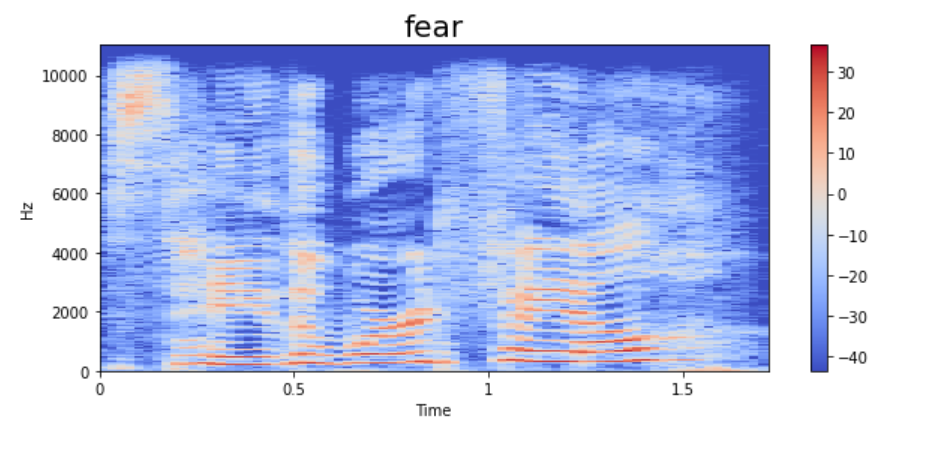
\includegraphics[width=0.5\textwidth]{spectrogram}
\caption{Spectrogram}
\end{figure}\\
We give the audio file path as input and get a feature as a numpy array.\\
\begin{figure}[h!]
\centering

\includegraphics[width=0.5\textwidth]{audio}
\caption{Audio}
\end{figure}\\
\begin{figure}[h!]
\centering
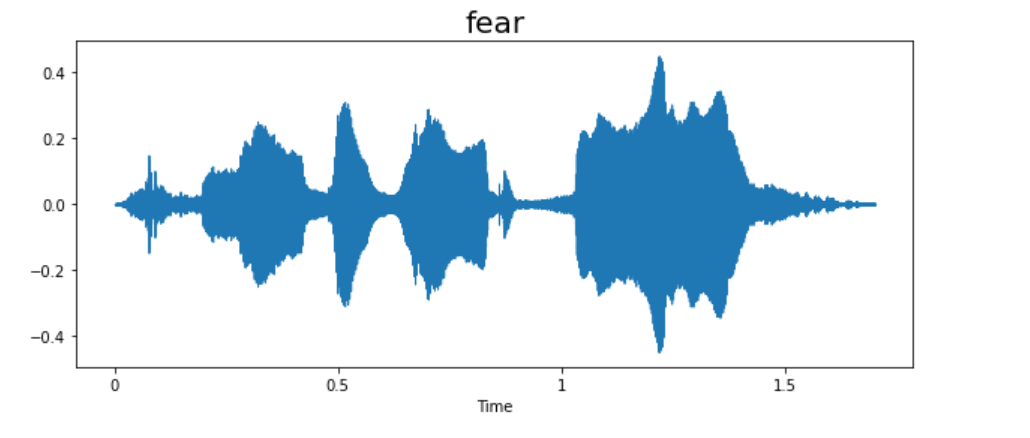
\includegraphics[width=0.5\textwidth]{wave_plot}
\caption{Wave Plot}
\end{figure}
Then these features are feeded into the deep learning based MLPClassifier for training.\\
The model learns from audio features. After training, when new audio is provided to the model it successfully predicts its emotion.\\
\begin{figure}[h!]
\centering
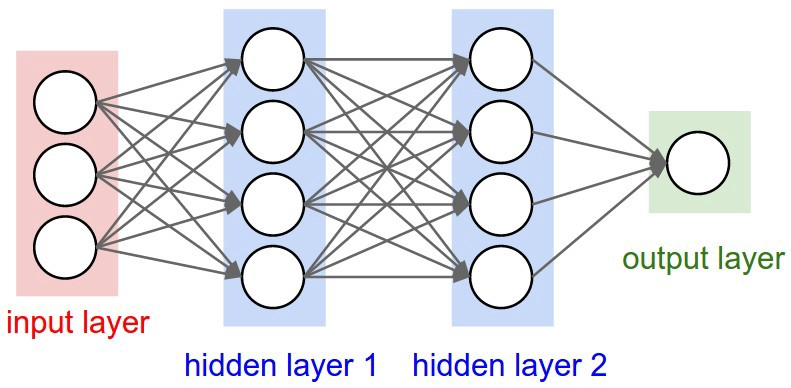
\includegraphics[width=0.5\textwidth]{deep_learning}
\caption{Deep Learning Model}
\end{figure}\\

\section{Result/Analysis/Accuracy}
Our proposed model attained an overall accuracy of 77\%.\\\\
We have also developed a web application for our project. Where user can select as well as record audio files and after giving that file to the system it will predict appropriate emotion.\\
\begin{figure}[h!]
\centering
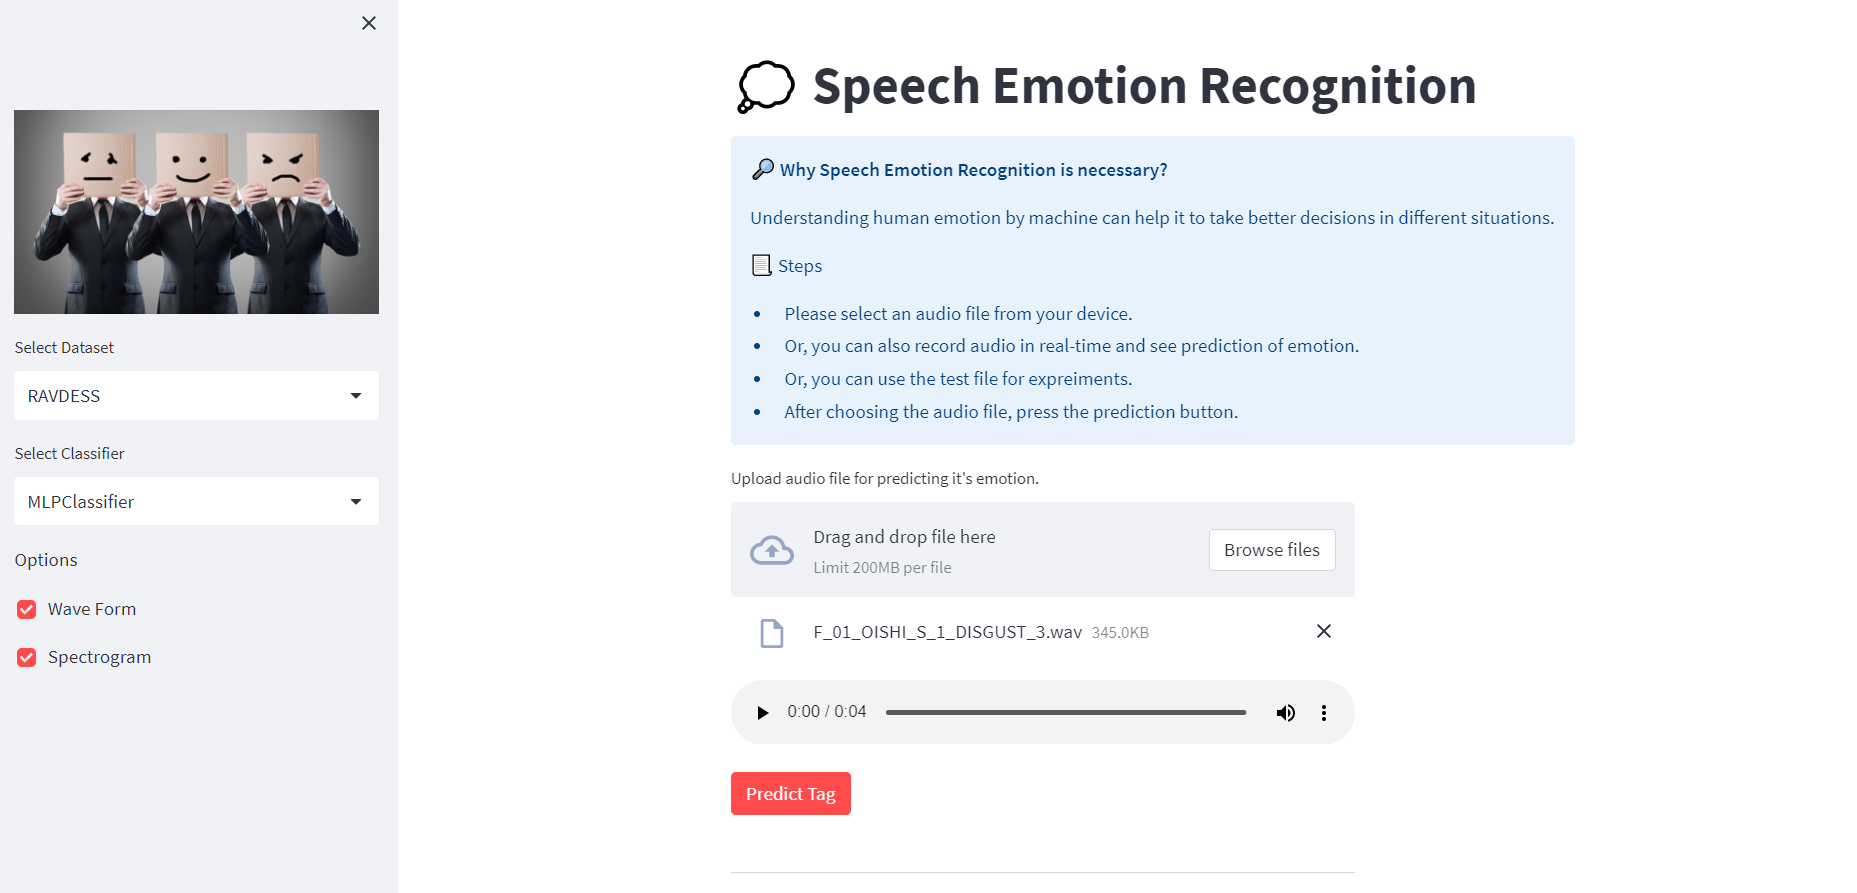
\includegraphics[width=0.5\textwidth]{webapp1}
\caption{Web Application 1}
\end{figure}\\
Here is the Web Application for selecting and recording audio for prediction of emotion.
\begin{figure}[h!]
\centering
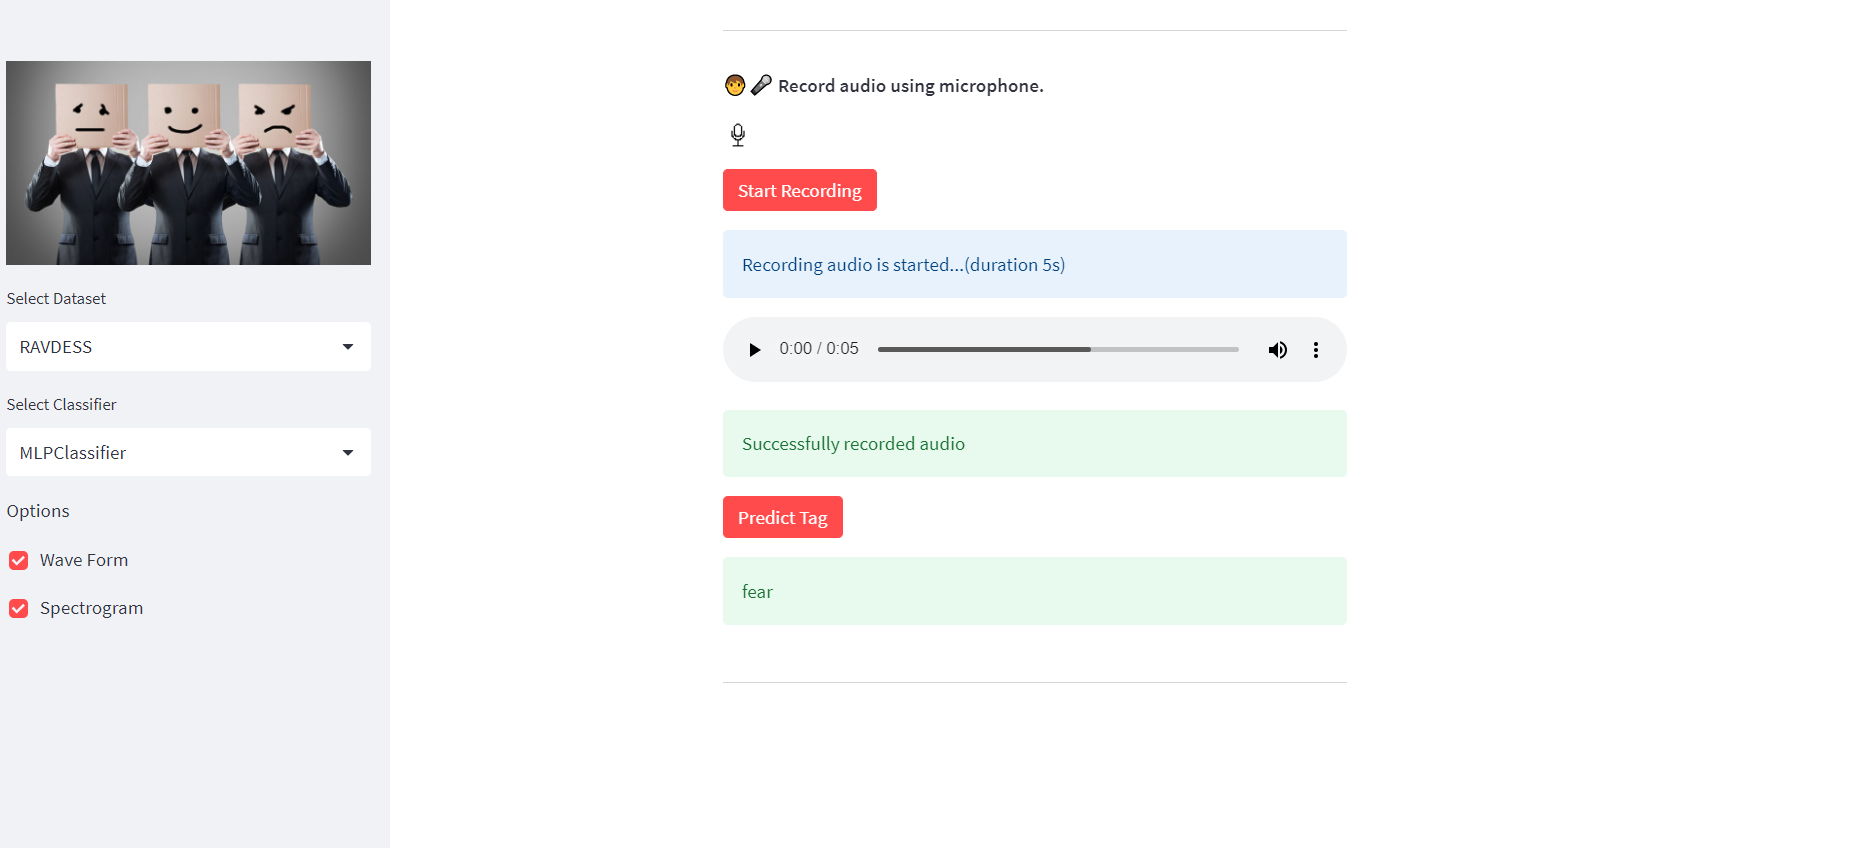
\includegraphics[width=0.5\textwidth]{webapp2}
\caption{Web Application 2}
\end{figure}\\

\section{Conclusion}
Our developed system can be used for different sectors such as call centers, tele-communication, tele-medicine etc. Also our proposed model can be used for Bangla Speech Emotion Recognition (SER). We hope, our work will encourage others to improve Bangla SER techniques and applications.

\bibliographystyle{plain}
\bibliography{references}

\end{document}


